\documentclass[12pt,a4paper]{article}

% ─── Page Layout ───────────────────────────────────────────────────────────────
\usepackage[a4paper, margin=0.8in, headheight=14pt]{geometry}

% ─── Fonts (XeLaTeX) ───────────────────────────────────────────────────────────
\usepackage{fontspec}
\usepackage{unicode-math}
\setmainfont{TeX Gyre Pagella}
\setmonofont[Scale=0.88]{TeX Gyre Cursor}
\setmathfont{Latin Modern Math}

% ─── Packages ──────────────────────────────────────────────────────────────────
\usepackage{xcolor}
\usepackage{colortbl}
\usepackage{titlesec}
\usepackage{enumitem}
\usepackage{tabularx}
\usepackage{booktabs}
\usepackage{array}
\usepackage{amsmath}
\usepackage{tikz}
\usetikzlibrary{shapes.geometric, arrows.meta, positioning, calc, fit, decorations.pathreplacing}
\usepackage{tcolorbox}
\tcbuselibrary{skins, breakable}
\usepackage{hyperref}
\usepackage{fancyhdr}
\usepackage{graphicx}
\usepackage{microtype}
\hyphenpenalty=10000
\exhyphenpenalty=10000
\sloppy
\usepackage{caption}
\usepackage{setspace}
\usepackage{multirow}
\usepackage{tocloft}

% ─── Q&A helper ────────────────────────────────────────────────────────────────
\newcommand{\Q}[1]{\textbf{#1}\par\noindent\ignorespaces}

% ─── Colour Palette ────────────────────────────────────────────────────────────
\definecolor{myred}{RGB}{196,30,58}
\definecolor{mydark}{RGB}{30,30,50}
\definecolor{mygreen}{RGB}{14,120,80}
\definecolor{myteal}{RGB}{0,130,140}
\definecolor{myamber}{RGB}{180,100,0}
\definecolor{mypurple}{RGB}{100,30,160}
\definecolor{mygray}{RGB}{246,247,249}
\definecolor{mgframe}{RGB}{180,185,200}
\definecolor{watermark}{RGB}{145,150,170}
\definecolor{hdrred}{RGB}{250,232,235}
\definecolor{hdrgreen}{RGB}{220,244,233}
\definecolor{hdrteal}{RGB}{220,242,244}
\definecolor{hdramber}{RGB}{253,242,215}
\definecolor{hdrpurple}{RGB}{238,228,255}
\definecolor{hdrgray}{RGB}{238,240,245}
\definecolor{rowalt}{RGB}{250,251,253}

% ─── Section Formatting ────────────────────────────────────────────────────────
\titleformat{\section}
  {\large\bfseries\color{myred}}{\thesection.}{0.5em}{}
  [\vspace{1pt}{\color{myred}\rule{\linewidth}{0.8pt}}]
\titleformat{\subsection}
  {\normalsize\bfseries\color{myteal}}{\thesubsection}{0.5em}{}
\titlespacing*{\section}{0pt}{18pt}{7pt}
\titlespacing*{\subsection}{0pt}{11pt}{4pt}

% ─── Paragraph ─────────────────────────────────────────────────────────────────
\setlength{\parindent}{0pt}
\setlength{\parskip}{4pt}

% ─── TOC Styling ───────────────────────────────────────────────────────────────
\renewcommand{\cfttoctitlefont}{\large\bfseries\color{myred}}
\renewcommand{\cftaftertoctitle}{\par\noindent{\color{myred}\rule{\linewidth}{0.8pt}}}
\setlength{\cftbeforetoctitleskip}{0pt}
\setlength{\cftaftertoctitleskip}{6pt}
\renewcommand{\cftsecfont}{\normalsize\bfseries\color{mydark}}
\renewcommand{\cftsecpagefont}{\normalsize\bfseries\color{mydark}}
\renewcommand{\cftsecleader}{\cftdotfill{\cftdotsep}}
\setlength{\cftbeforesecskip}{7pt}
\renewcommand{\cftsubsecfont}{\small\color{mydark}}
\renewcommand{\cftsubsecpagefont}{\small\color{mydark}}
\setlength{\cftbeforesubsecskip}{3pt}
\setlength{\cftsubsecindent}{1.4em}

% ─── Table helpers ─────────────────────────────────────────────────────────────
\renewcommand{\arraystretch}{1.45}
\setlength{\tabcolsep}{6pt}
\arrayrulecolor{mydark}
\newcolumntype{B}[1]{>{\small\bfseries\raggedright\arraybackslash}m{#1}}
\newcolumntype{Y}{>{\small\raggedright\arraybackslash}X}
\renewcommand{\tabularxcolumn}[1]{m{#1}}

% ─── Header / Footer ───────────────────────────────────────────────────────────
\pagestyle{fancy}
\fancyhf{}
\fancyhead[L]{\small\color{myred}\textbf{OE-EC604B}\;\color{mydark}--- Operating System}
\fancyhead[R]{\small\color{myteal}\textbf{Module 4 Notes}}
\fancyfoot[C]{\small\color{mydark}\thepage}
\fancyfoot[R]{\small\color{watermark}\textit{\copyright\ Biraj}}
\renewcommand{\headrulewidth}{0.5pt}
\renewcommand{\footrulewidth}{0.3pt}

% ─── Hyperref ──────────────────────────────────────────────────────────────────
\hypersetup{
  colorlinks=true, linkcolor=myteal, urlcolor=myteal,
  pdfauthor={Biraj Sarkar},
  pdftitle={OE-EC604B --- Module 4 Notes}
}

% ─── tcolorbox styles ──────────────────────────────────────────────────────────
\tcbset{
  tikzbox/.style={
    colback=mygray, colframe=mgframe, boxrule=0.6pt, arc=4pt,
    left=8pt, right=8pt, top=6pt, bottom=6pt,
    colbacktitle=mgframe, coltitle=mydark,
    fonttitle=\small\bfseries
  },
  defbox/.style={
    colback=hdrgreen, colframe=mygreen, boxrule=0.8pt, arc=4pt,
    left=9pt, right=9pt, top=6pt, bottom=6pt,
    colbacktitle=mygreen, coltitle=white,
    fonttitle=\small\bfseries
  },
  formulabox/.style={
    colback=hdrteal, colframe=myteal, boxrule=0.8pt, arc=4pt,
    left=9pt, right=9pt, top=7pt, bottom=7pt,
    colbacktitle=myteal, coltitle=white,
    fonttitle=\small\bfseries
  },
  examplebox/.style={
    colback=hdramber, colframe=myamber, boxrule=0.8pt, arc=4pt,
    left=9pt, right=9pt, top=6pt, bottom=6pt,
    colbacktitle=myamber, coltitle=white,
    fonttitle=\small\bfseries
  },
  masonbox/.style={
    colback=hdrpurple, colframe=mypurple, boxrule=0.8pt, arc=4pt,
    left=9pt, right=9pt, top=6pt, bottom=6pt,
    colbacktitle=mypurple, coltitle=white,
    fonttitle=\small\bfseries
  },
  exambox/.style={
    colback=hdrpurple, colframe=mypurple, boxrule=1pt, arc=5pt,
    left=10pt, right=10pt, top=8pt, bottom=8pt,
    colbacktitle=mypurple, coltitle=white,
    fonttitle=\bfseries,
    breakable, title after break={\textbf{Frequently Asked / Viva Questions (contd.)}}}
}
% Make all boxes breakable across pages
\tcbset{breakable}

% ─── TikZ styles ───────────────────────────────────────────────────────────────
\tikzset{
  block/.style={rectangle, draw=myteal, fill=hdrteal,
    text width=2.4cm, align=center, minimum height=0.95cm,
    font=\small, rounded corners=3pt, line width=0.7pt},
  redblock/.style={rectangle, draw=myred, fill=hdrred,
    text width=2.4cm, align=center, minimum height=0.95cm,
    font=\small, rounded corners=3pt, line width=0.7pt},
  greenblock/.style={rectangle, draw=mygreen, fill=hdrgreen,
    text width=2.4cm, align=center, minimum height=0.95cm,
    font=\small, rounded corners=3pt, line width=0.7pt},
  amberblock/.style={rectangle, draw=myamber, fill=hdramber,
    text width=2.4cm, align=center, minimum height=0.95cm,
    font=\small, rounded corners=3pt, line width=0.7pt},
  purpblock/.style={rectangle, draw=mypurple, fill=hdrpurple,
    text width=2.4cm, align=center, minimum height=0.95cm,
    font=\small, rounded corners=3pt, line width=0.7pt},
  sumjunc/.style={circle, draw=myamber, fill=hdramber,
    minimum size=0.62cm, font=\small, line width=0.8pt},
  arrow/.style={-Stealth, thick, color=mydark},
  redarrow/.style={-Stealth, thick, color=myred},
  line/.style={thick, color=mydark}
}

% ═══════════════════════════════════════════════════════════════════════════════
\begin{document}
% ═══════════════════════════════════════════════════════════════════════════════

\begin{center}
  {\LARGE\bfseries\color{myred} OE-EC604B --- Operating System}\\[5pt]
  {\normalsize\color{mydark} Semester VI \quad$\bullet$\quad 3L:0T:0P \quad$\bullet$\quad 3 Credits}\\[3pt]
  {\normalsize\color{myteal}\textbf{Module 4 Exam Notes: CPU Scheduling}}\\[3pt]
  {\small\color{mydark} CGEC \;$|$\; B.Tech ECE (2023--27) \;$|$\; \textit{Biraj Sarkar}}
\end{center}
\vspace{2pt}
\noindent{\color{myred}\rule{\linewidth}{1.5pt}}
\vspace{2pt}

\hypersetup{linkcolor=mydark}
\tableofcontents
\hypersetup{linkcolor=myteal}
\newpage

% ===============================================================================
\section{Scheduling Concepts and Performance Criteria}
% ===============================================================================

In a single-processor system, only one process can run at a time; others must wait until the CPU is free. The objective of multiprogramming is to run multiple processes concurrently to maximize CPU utilization.

\subsection{CPU-I/O Burst Cycle}
Process execution consists of a cycle of \textbf{CPU execution (CPU burst)} and \textbf{I/O wait (I/O burst)}. Processes alternate between these two states.
\begin{itemize}[leftmargin=*, itemsep=3pt]
  \item \textbf{CPU-bound Process:} Spends most of its time doing computations (long CPU bursts).
  \item \textbf{I/O-bound Process:} Spends most of its time waiting for I/O (short CPU bursts).
\end{itemize}

\subsection{Scheduling Criteria}
Operating systems select processes from the ready queue based on five key performance criteria:
1. \textbf{CPU Utilization:} The percentage of time the CPU is busy executing tasks (Goal: Maximize, 40\% to 90\%).
2. \textbf{Throughput:} The number of processes completed per unit time (Goal: Maximize).
3. \textbf{Turnaround Time ($TAT$):} The total interval from process submission to its completion (Goal: Minimize).
4. \textbf{Waiting Time ($WT$):} The total time a process spends waiting in the ready queue (Goal: Minimize).
5. \textbf{Response Time ($RT$):} The time from submission to the first CPU response (Goal: Minimize, critical for interactive systems).

% ===============================================================================
\section{CPU Scheduling Algorithms}
% ===============================================================================

CPU scheduling decisions take place under four conditions:
1. When a process switches from running to waiting (Non-Preemptive).
2. When a process switches from running to ready (Preemptive).
3. When a process switches from waiting to ready (Preemptive).
4. When a process terminates (Non-Preemptive).

\subsection{First-Come, First-Served (FCFS)}
\begin{itemize}[leftmargin=*, itemsep=3pt]
  \item \textbf{Principle:} The process that requests the CPU first gets it first. Managed via a FIFO queue.
  \item \textbf{Drawback:} Non-preemptive. Suffers from the \textbf{Convoy Effect} --- short processes must wait for a single long process to finish, causing high average waiting times.
\end{itemize}

\subsection{Shortest Job First (SJF)}
\begin{itemize}[leftmargin=*, itemsep=3pt]
  \item \textbf{Principle:} Associates with each process the length of its next CPU burst. The process with the shortest burst is scheduled.
  \item \textbf{SJF (Non-preemptive):} Once CPU is allocated, it cannot be preempted.
  \item \textbf{SRTF (Preemptive SJF):} If a new process arrives with a shorter remaining burst than the currently running process, the CPU is preempted.
  \item \textbf{Advantage:} SJF is \textbf{optimal} --- it gives the minimum average waiting time for a given set of processes.
  \item \textbf{Disadvantage:} Cannot be implemented directly because the length of the next CPU burst is unknown. Prone to \textbf{starvation} of long processes.
\end{itemize}

\subsection{Round Robin (RR) Scheduling}
\begin{itemize}[leftmargin=*, itemsep=3pt]
  \item \textbf{Principle:} Designed for time-sharing systems. The CPU scheduler goes around the ready queue, allocating the CPU to each process for a time interval up to \textbf{1 time quantum (slice)} ($q$).
  \item \textbf{Working:} If process burst $> q$, it is preempted and put back at the tail of the ready queue.
  \item \textbf{Performance Dependency:} If $q$ is extremely large, RR behaves like FCFS. If $q$ is extremely small, it causes high context-switching overhead.
\end{itemize}

\subsection{Priority Scheduling}
\begin{itemize}[leftmargin=*, itemsep=3pt]
  \item \textbf{Principle:} A priority number is associated with each process, and the CPU is allocated to the process with the highest priority (lowest integer usually represents highest priority).
  \item \textbf{Problem:} \textbf{Starvation (Indefinite Blocking)} of low-priority processes.
  \item \textbf{Solution:} \textbf{Aging} --- gradually increasing the priority of processes that wait in the system for a long time.
\end{itemize}

\subsection{Multilevel Queue (MLQ) \& Multilevel Feedback Queue (MLFQ)}
\begin{itemize}[leftmargin=*, itemsep=3pt]
  \item \textbf{MLQ:} Partitioned ready queue into several separate queues (e.g., foreground interactive and background batch) with fixed priority. No movement between queues.
  \item \textbf{MLFQ:} Allows processes to move between queues based on CPU burst history. If a process uses too much CPU time, it is demoted. If it waits too long, it is promoted (aging).
\end{itemize}

\begin{tcolorbox}[tikzbox, title={Multilevel Feedback Queue Structure}]
\centering
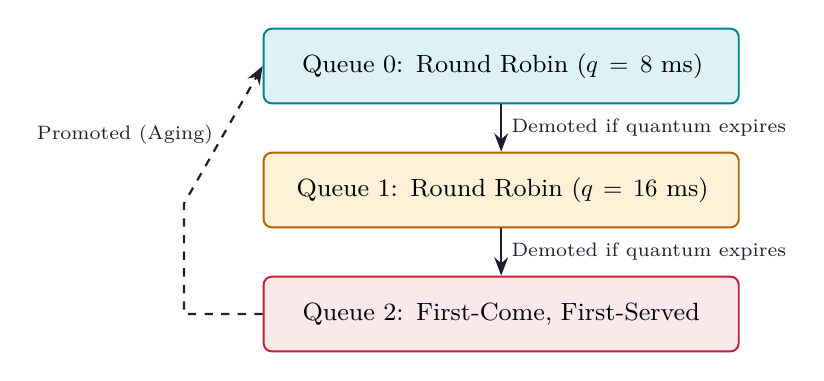
\begin{tikzpicture}[node distance=0.8cm, thick, font=\small]
  \node[block, text width=5.8cm, fill=hdrteal, draw=myteal] (q0) {Queue 0: Round Robin ($q = 8$ ms)};
  \node[block, text width=5.8cm, fill=hdramber, draw=myamber, below=0.6cm of q0] (q1) {Queue 1: Round Robin ($q = 16$ ms)};
  \node[block, text width=5.8cm, fill=hdrred, draw=myred, below=0.6cm of q1] (q2) {Queue 2: First-Come, First-Served};

  \draw[arrow] (q0.south) -- node[right, font=\scriptsize] {Demoted if quantum expires} (q1.north);
  \draw[arrow] (q1.south) -- node[right, font=\scriptsize] {Demoted if quantum expires} (q2.north);
  \draw[arrow, dashed] (q2.west) -- ++(-1.0, 0) -- ++(0, 1.4) -- node[left, font=\scriptsize] {Promoted (Aging)} (q0.west);
\end{tikzpicture}
\end{tcolorbox}

% ===============================================================================
\section{Multiprocessor Scheduling}
% ===============================================================================

When multiple CPUs are available, scheduling complexity increases:
\begin{itemize}[leftmargin=*, itemsep=3pt]
  \item \textbf{Asymmetric Multiprocessing:} One master processor handles all scheduling decisions, I/O processing, and system activities; others run only user code. Simple, but master is a bottleneck.
  \item \textbf{Symmetric Multiprocessing (SMP):} Each processor schedules itself from the common ready queue or private ready queue.
  \item \textbf{Processor Affinity:} A process has an affinity for the processor it is currently running on to avoid the cache invalidation cost of migrating to another CPU.
  \begin{itemize}[leftmargin=*, itemsep=2.5pt, topsep=0pt]
    \item *Soft Affinity:* OS tries to keep process on same CPU but does not guarantee it.
    \item *Hard Affinity:* Process specifies it can only run on a subset of CPUs.
  \end{itemize}
  \item \textbf{Load Balancing:} Keeps workload evenly distributed across all CPUs.
  \begin{itemize}[leftmargin=*, itemsep=2.5pt, topsep=0pt]
    \item *Push Migration:* A specific task monitors load and pushes processes from overloaded CPUs to idle ones.
    \item *Pull Migration:* An idle processor pulls a waiting task from a busy processor.
    \end{itemize}
  \end{itemize}

\newpage
% ===============================================================================
% MANDATORY QUICK REVISION PAGE
% ===============================================================================
\begin{center}
  {\large\bfseries\color{myred} Quick Revision --- Module 4}\\[3pt]
  {\small\color{mydark} CPU Scheduling $|$ OE-EC604B}
\end{center}
\noindent{\color{myred}\rule{\linewidth}{1.2pt}}
\vspace{4pt}

\begin{tcolorbox}[formulabox, title={\textbf{Core Scheduling Formulas}}]
$$\text{Turnaround Time (TAT)} = \text{Completion Time (CT)} - \text{Arrival Time (AT)}$$
$$\text{Waiting Time (WT)} = \text{Turnaround Time (TAT)} - \text{Burst Time (BT)}$$
$$\text{Response Time (RT)} = \text{First CPU Start Time} - \text{Arrival Time (AT)}$$
$$\text{Average Waiting Time} = \frac{1}{N}\sum_{i=1}^{N} WT_i$$
\end{tcolorbox}

\begin{tcolorbox}[defbox, title={\textbf{One-Line Definitions}}]
\begin{itemize}[leftmargin=*, itemsep=2.5pt, topsep=0pt]
  \item \textbf{Throughput:} Number of completed processes per unit time.
  \item \textbf{Convoy Effect:} Scenario in FCFS where short jobs wait behind a very long job, degrading latency.
  \item \textbf{Preemptive Scheduling:} OS mechanism to interrupt a running process and assign CPU to another.
  \item \textbf{Quantum ($q$):} The fixed time slice allocated to a process in Round Robin scheduling.
  \item \textbf{Starvation:} Situation where a process waits indefinitely because other processes have higher priorities.
  \item \textbf{Aging:} Technique of gradually increasing the priority of waiting processes to prevent starvation.
  \item \textbf{Processor Affinity:} Cache optimization keeping a process executing on the same CPU core.
  \item \textbf{Symmetric Multiprocessing (SMP):} Multiprocessing where each CPU makes its own scheduling decisions.
\end{itemize}
\end{tcolorbox}

\begin{tcolorbox}[exambox, title={\textbf{Frequently Asked / Viva Questions}}]
\begin{enumerate}[topsep=0pt, label=\textbf{Q\arabic*.}, itemsep=5pt]
  \item \Q{Compare FCFS, SJF, and Round Robin scheduling algorithms.}
    FCFS is simple, non-preemptive, but prone to convoy effect. SJF is optimal for average waiting time but causes starvation and is hard to predict. Round Robin is preemptive, quantum-based, and ideal for interactive systems.
  \item \Q{Show the Gantt chart and compute Turnaround and Waiting times for:}\\
    \begin{tabularx}{\linewidth}{|B{1.5cm}|Y|Y|Y|}
    \hline
    Process & Arrival Time & Burst Time & Priority \\
    \hline
    P1 & 0 & 8 & 3 (Low) \\
    P2 & 1 & 4 & 1 (High) \\
    P3 & 2 & 2 & 2 \\
    \hline
    \end{tabularx}\\
    \textbf{Using Preemptive Priority Scheduling:}\par
    *Gantt Chart:* P1 runs from [0-1]. At $t=1$, P2 arrives with priority 1, preempts P1. P2 runs from [1-5]. At $t=5$, P3 runs from [5-7]. At $t=7$, P1 finishes from [7-14].\par
    *Completion Times (CT):* P2 = 5, P3 = 7, P1 = 14.\par
    *Turnaround Times (TAT = CT - AT):* P1 = 14, P2 = 4, P3 = 5. (Avg TAT = 7.67).\par
    *Waiting Times (WT = TAT - BT):* P1 = 6, P2 = 0, P3 = 3. (Avg WT = 3.0).
  \item \Q{What is the Convoy Effect in CPU scheduling? How is it resolved?}
    It happens in FCFS when one CPU-bound process holds the CPU while multiple I/O-bound processes wait in the ready queue. Resolved by using preemptive scheduling algorithms (like Round Robin).
  \item \Q{Why is SJF scheduling called "optimal"? Why is it difficult to implement?}
    It is optimal because it mathematically minimizes the average waiting time for a set of processes. It is hard to implement because the exact burst time of future processes cannot be known in advance (it must be estimated using exponential smoothing).
  \item \Q{How does the performance of Round Robin scheduling depend on the time quantum?}
    If the quantum is too large, it degenerates into FCFS. If it is too small, it causes excessive context-switching overhead, which wastes CPU cycles. A rule of thumb is that 80\% of CPU bursts should be shorter than the quantum.
  \item \Q{What is starvation? How does aging solve it?}
    Starvation occurs when low-priority processes never get scheduled because high-priority processes keep arriving. Aging solves this by gradually increasing the priority of a process the longer it remains waiting in the ready queue.
  \item \Q{Differentiate between Multilevel Queue (MLQ) and Multilevel Feedback Queue (MLFQ).}
    In MLQ, processes are permanently assigned to a queue based on type, with no queue switching. In MLFQ, processes can move dynamically between queues based on CPU behavior, enabling automatic detection of I/O vs CPU bound jobs.
  \item \Q{Explain Processor Affinity and its types.}
    Processor affinity is the policy of keeping a process on the same CPU to leverage cached data. Soft affinity means the OS tries to enforce this but can migrate the process. Hard affinity guarantees the process runs only on designated CPUs.
  \item \Q{What is the difference between Push and Pull migration in load balancing?}
    Push migration runs a task that periodically checks load and "pushes" processes from busy CPUs to idle ones. Pull migration occurs when an idle CPU queries other CPUs and "pulls" an waiting process to execute.
  \item \Q{Explain CPU-I/O burst cycle.}
    A process's lifecycle alternates between CPU execution blocks (CPU bursts) and waiting for device I/O actions (I/O bursts), ending with a final CPU burst and termination request.
\end{enumerate}
\end{tcolorbox}

\begin{tcolorbox}[tikzbox, title={CPU Scheduling Algorithms Comparison}]
\renewcommand{\arraystretch}{1.4}
\par\noindent
\begin{tabularx}{\linewidth}{|B{2.2cm}|>{\small\centering\arraybackslash}X|>{\small\centering\arraybackslash}X|>{\small\centering\arraybackslash}X|}
\hline
\textbf{Algorithm} & \textbf{\color{myred}Preemptive?} & \textbf{\color{myteal}Starvation Risk?} & \textbf{\color{myamber}Optimal average WT?} \\
\hline
\textbf{FCFS} & No & No & No \\
\hline
\textbf{SJF} & No & Yes & Yes (among non-preemptive) \\
\hline
\textbf{SRTF} & Yes & Yes & Yes (optimal) \\
\hline
\textbf{Round Robin} & Yes & No & No \\
\hline
\textbf{Priority} & Yes/No & Yes & No \\
\hline
\end{tabularx}
\end{tcolorbox}

\end{document}
